%----------------------------------------------------------------------------------------
%    PACKAGES AND THEMES
%----------------------------------------------------------------------------------------

\documentclass[xcolor=dvipsnames]{beamer}
\usetheme{SimpleDarkBlue}

\usepackage{hyperref}
\usepackage{graphicx} % Allows including images
\usepackage{booktabs} % Allows the use of \toprule, \midrule and \bottomrule in tables
\usepackage{lastpage} % Utiliser le package pour personnaliser le pied de page
\usepackage{amsmath}
\usepackage{amssymb}
\usepackage{tikz}
\usepackage[utf8]{inputenc}
\usepackage[T1]{fontenc}
\usepackage{array}
\usepackage{listings}
\usepackage{minted}
\usepackage{caption}
\usetikzlibrary{arrows.meta}
\usepackage{xcolor}
\usepackage{comment}
\usepackage{seqsplit}

\definecolor{myorange}{HTML}{A86229}
\definecolor{mygreen}{HTML}{4C7743}
\definecolor{mycomment}{HTML}{75A300}

\lstdefinestyle{pythonStyle}{
  language=Python,
  basicstyle=\ttfamily\tiny\color{black},       % police tiny et couleur noire
  backgroundcolor=\color{white},                % fond blanc
  keywordstyle=\color{myorange}\bfseries,          % mots-clés en noir gras
  commentstyle=\color{mycomment},                    % commentaires en gris
  stringstyle=\color{mygreen},                    % chaînes en noir
  showstringspaces=false,                       % ne montre pas les espaces
  breaklines=true,                              % coupe les longues lignes
  breakatwhitespace=true,                       % coupe à un espace
  numbers=left,                                 % numérotation des lignes à gauche
  numberstyle=\tiny\color{gray},                % style des numéros de ligne
  stepnumber=1,                                 % numéroter chaque ligne
  frame=none,                                   % pas de cadre
  tabsize=2,                                     % petite indentation
  aboveskip=2pt, belowskip=2pt,                 % peu d’espace autour du bloc
  literate= {é}{{\'e}}1 {è}{{\`e}}1 {ê}{{\^e}}1 {ë}{{\"e}}1 {à}{{\`a}}1 {â}{{\^a}}1 {ä}{{\"a}}1 {ù}{{\`u}}1 {û}{{\^u}}1 {ü}{{\"u}}1 {î}{{\^i}}1 {ï}{{\"i}}1 {ô}{{\^o}}1 {ö}{{\"o}}1 {ç}{{\c{c}}}1 {É}{{\'E}}1 {À}{{\`A}}1 {Ç}{{\c{C}}}1  % les accents
}


%\captionsetup[figure]{labelformat=simple} % Active la numérotation des figures

%\addtobeamertemplate{caption}{}{} % Enlève tout ajout de Beamer à la caption
%\renewcommand{\figurename}{}      % Vide le nom "Figure"

%----------------------------------------------------------------------------------------
%    TITLE PAGE
%----------------------------------------------------------------------------------------


\title{Compression d'images avec pertes}
\subtitle{Maximilien Dubus \ \ \textbf{·} \ \ MPI \ \ \textbf{·} \ \ Candidat 16078}


\date{ } % Date, can be changed to a custom date


% Redéfinir le pied de page avec les éléments spécifiés
\setbeamertemplate{footline}{
  \ifnum\value{framenumber}>1 % Vérifie si le numéro de la diapositive est supérieur à 1
    \leavevmode%
    \hbox{%
    \begin{beamercolorbox}[wd=.25\paperwidth,ht=2.25ex,dp=1ex,center]{author in head/foot}%
      \usebeamerfont{author in head/foot} Maximilien Dubus
    \end{beamercolorbox}%
    \begin{beamercolorbox}[wd=.5\paperwidth,ht=2.25ex,dp=1ex,center]{title in head/foot}%
      \usebeamerfont{title in head/foot} Compression d'images
    \end{beamercolorbox}%
    \begin{beamercolorbox}[wd=.25\paperwidth,ht=2.25ex,dp=1ex,center]{date in head/foot}%
      \usebeamerfont{date in head/foot}Candidat 16078 \hfill
      \ifnum\value{framenumber}<31
        \textbf{\insertframenumber{/30}}
      \else
        \textbf{\insertframenumber{}/\pageref{LastPage}}
      \fi
    \end{beamercolorbox}}%
    \vskip0pt%
  \fi
}

% Supprimer les icônes de navigation
\setbeamertemplate{caption}{\insertcaption}
\setbeamertemplate{caption}[numbered]

\definecolor{mycustomcolor}{HTML}{0D2659} % Code hexadécimal pour une couleur bleue
\setbeamercolor{block title}{bg=mycustomcolor,fg=white} % Appliquer cette couleur aux titres de bloc


%----------------------------------------------------------------------------------------
%    PRESENTATION SLIDES
%----------------------------------------------------------------------------------------

\begin{document}

\begin{frame}
    \begin{tikzpicture}[remember picture, overlay]
        \node[anchor=center] at (current page.center) {
            \includegraphics[width=\paperwidth, height=\paperheight]{rosier_degrade4.png}
        };
    \end{tikzpicture}
    
    \vspace{-100pt}
    \titlepage
\end{frame}

\begin{frame}{Introduction}
    \centering
    % https://www.blogdumoderateur.com/chiffres-instagram/
    100 000 000 de photos sont publiées chaque jour sur Instagram. \\
    \footnotesize
    \[
        \underbrace{100\,000\,000}_{\shortstack{\text{nombre de}\\\text{photos}}}
        \times
        \underbrace{2\,000 \times 1\,000}_{\shortstack{\text{\small nombre de}\\\text{pixels par photo}}}
        \times
        \underbrace{3}_{\shortstack{\text{nombre d'octets}\\\text{par pixel}}}
        =  600\ \text{To}
    \]

\end{frame}

%------------------------------------------------
\section{La compression JPEG}
%------------------------------------------------


\begin{frame} {Transformation des couleurs}
    \begin{figure}
        \centering
        \begin{tikzpicture}
            % Inclure l'image
            \node[anchor=south west,inner sep=0] (image) at (0,0) {
                \includegraphics[width=1\linewidth, trim=0cm 25cm 0cm 0cm, clip]{Compression_JPEG.png}
            };
            % Dessiner un carré rouge
            \begin{scope}[x={(image.south east)},y={(image.north west)}]
                % Coordonnées du carré : (x, y) pour le coin inférieur gauche
                \draw[red,ultra thick] (0.155,0.02) rectangle (0.275,0.98);
            \end{scope}
        \end{tikzpicture}
        %\caption{Étapes de la compression JPEG}
    \end{figure}
\end{frame}

\begin{frame}{Transformation des couleurs}

    \begin{columns}

        \begin{column}{0.4\textwidth}
            \tiny
            \begin{align*}
                Y &= 0,299 \, R + 0,587 \, V + 0,114 \, B \\
                Cb &= -0,1687 \, R - 0,3313 \, V + 0,5 \, B + 128 \\
                Cr &= 0,5 \, R - 0,4187 \, V - 0,0813 \, B + 128
            \end{align*}
            \begin{figure}
                \centering
                \includegraphics[width=1\linewidth]{principale_1000_750_smooth.jpg}
                \caption{Image Originale}
            \end{figure}
        \end{column}
        
        \begin{column}{0.3\textwidth}
            \vspace{-15pt}
            \begin{figure}
                \centering
                \includegraphics[width=0.8\linewidth]{rouge.jpg}
            \end{figure}
            \vspace{-15pt}
            \begin{figure}
                \centering
                \includegraphics[width=.8\linewidth]{vert.jpg}
            \end{figure}
            \vspace{-15pt}
            \begin{figure}
                \centering
                \includegraphics[width=.8\linewidth]{bleu.jpg}
                \caption{\centering Décomposée \\ en R V B}
            \end{figure}
        \end{column}

        \begin{column}{0.3\textwidth}
            \vspace{-15pt}
            \begin{figure}
                \centering
                \includegraphics[width=.8\linewidth]{luminance.jpg}
            \end{figure}
            \vspace{-15pt}
            \begin{figure}
                \centering
                \includegraphics[width=.8\linewidth]{chrominance_bleu.jpg}
            \end{figure}
            \vspace{-15pt}
            \begin{figure}
                \centering
                \includegraphics[width=.8\linewidth]{chrominance_rouge.jpg}
                \caption{\centering Décomposée \\ en Y Cb Cr}
            \end{figure}
        \end{column}
        
    \end{columns}
    
\end{frame}


\begin{frame} {Sous-échantillonnage de la chrominance}
    \begin{figure}
        \centering
        \begin{tikzpicture}
            % Inclure l'image
            \node[anchor=south west,inner sep=0] (image) at (0,0) {
                \includegraphics[width=1\linewidth, trim=0cm 25cm 0cm 0cm, clip]{Compression_JPEG.png}
            };
            % Dessiner un carré rouge
            \begin{scope}[x={(image.south east)},y={(image.north west)}]
                % Coordonnées du carré : (x, y) pour le coin inférieur gauche
                \draw[red,ultra thick] (0.3,0.02) rectangle (0.42,0.98);
            \end{scope}
        \end{tikzpicture}
        %\caption{Étapes de la compression JPEG}
    \end{figure}
\end{frame}


\begin{frame}{Sous-échantillonnage de la chrominance}

\centering
    \scriptsize

    \setbeamerfont{caption}{size=\scriptsize}
    \setbeamerfont{caption name}{size=\scriptsize}

    \begin{figure}
        \centering
        \includegraphics[width=4.7cm,height=1.76cm]{cbcr.jpg}
        \caption{les deux matrices de chrominance}
    \end{figure}
        
    \vspace{-7pt}

    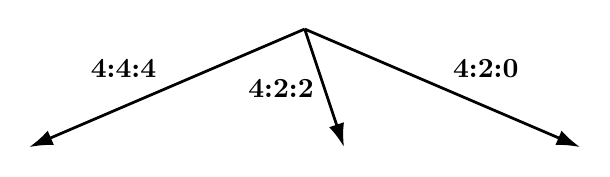
\begin{tikzpicture}
            
        \draw[-{Latex[length=3mm, width=2mm]}, line width=1pt] (1,2) -- (-2.5,.5) node[midway, above left] {\textbf{4:4:4}};

        \draw[-{Latex[length=3mm, width=2mm]}, line width=1pt] (1,2) -- (1.5,.5) node[midway, left] {\textbf{4:2:2}};
        
        \draw[-{Latex[length=3mm, width=2mm]}, line width=1pt] (1,2) -- (4.5,.5) node[midway, above right] {\textbf{4:2:0}};

    \end{tikzpicture}

    \vspace{7pt}


    \begin{minipage}{0.42\textwidth}
        \vspace{-9pt}
        \begin{figure}
            \centering
            \includegraphics[width=4.7cm,height=1.76cm]{cbcr.jpg}
            \caption*{\centering on garde \textbf{toute} l'information}
        \end{figure}
    \end{minipage}
    \hfill
    \begin{minipage}{0.28\textwidth}
        \begin{figure}
            \centering
            \includegraphics[width=2.35cm,height=1.76cm]{cbcr.jpg}
            \caption*{\centering on garde \textbf{la moitié} de l'information}
        \end{figure}
    \end{minipage}
    \hfill
    \begin{minipage}{0.28\textwidth}
        \begin{figure}
            \centering
            \includegraphics[width=2.35cm,height=0.88cm]{cbcr.jpg}
            \caption*{\centering on garde \textbf{un quart} de l'information}
        \end{figure}
    \end{minipage}
    \hfill

\end{frame}

\begin{frame} {Découpage en matrices 8x8}
    \begin{figure}
        \centering
        \begin{tikzpicture}
            % Inclure l'image
            \node[anchor=south west,inner sep=0] (image) at (0,0) {
                \includegraphics[width=1\linewidth, trim=0cm 25cm 0cm 0cm, clip]{Compression_JPEG.png}
            };
            % Dessiner un carré rouge
            \begin{scope}[x={(image.south east)},y={(image.north west)}]
                % Coordonnées du carré : (x, y) pour le coin inférieur gauche
                \draw[red,ultra thick] (0.445,0.02) rectangle (0.563,0.98);
            \end{scope}
        \end{tikzpicture}
        %\caption{Étapes de la compression JPEG}
    \end{figure}
\end{frame}


\begin{frame}{Découpage en matrices 8$\times$8}
    % explication des hautes/basses fréquences

    \begin{columns}

        \begin{column}{0.42\textwidth}
            \vspace{-80pt}
            \begin{figure}
                \centering
                \includegraphics[width=1\linewidth]{luminance.jpg}
                \caption{\centering la luminance}
            \end{figure}
        \end{column}
        
        \begin{column}{0.58\textwidth}
            \begin{figure}
                \centering
                \includegraphics[width=.4\linewidth]{bloc_88.png}
                %\vspace{-7pt}
                \caption{\centering une matrice 8$\times$8 extraite}
            \end{figure}
            \vspace{-15pt}
            \begin{figure}
                \centering
                \includegraphics[width=.4\linewidth]{mat88_genere_aleatoirement3.png}
                \caption{\centering une matrice générée aléatoirement}
            \end{figure}
        \end{column}
        
    \end{columns}

    \begin{tikzpicture}[overlay, remember picture]
        % Dessiner un trait rouge
        \draw[red, thick] (current page.south west) ++(7.702cm,5.315cm) -- ++(-4.245cm,1.97cm);
        
        \draw[red, thick] (current page.south west) ++(7.702cm,7.932cm) -- ++(-4.245cm,-0.62cm);
        
        % Dessiner un carré rouge
        \draw[red, thick] (current page.south west) ++(7.702cm,5.315cm) rectangle ++(2.617cm,2.617cm);
    \end{tikzpicture}
    
\end{frame}


\begin{frame} {Transformée en cosinus discrète}
    \begin{figure}
        \centering
        \begin{tikzpicture}
            % Inclure l'image
            \node[anchor=south west,inner sep=0] (image) at (0,0) {
                \includegraphics[width=1\linewidth, trim=0cm 25cm 0cm 0cm, clip]{Compression_JPEG.png}
            };
            % Dessiner un carré rouge
            \begin{scope}[x={(image.south east)},y={(image.north west)}]
                % Coordonnées du carré : (x, y) pour le coin inférieur gauche
                \draw[red,ultra thick] (0.591,0.02) rectangle (0.71,0.98);
            \end{scope}
        \end{tikzpicture}
        %\caption{Étapes de la compression JPEG}
    \end{figure}
\end{frame}



\begin{frame}{Transformée en cosinus discrète unidimensionnelle}

    \centering
    DCT unidimensionnelle
    \small
    \[
        X_k = \sqrt{\dfrac{2}{N}}c(k)\sum_{n=0}^{N-1} x_n \cos \left( \frac{k\pi}{N} \left( n + \frac{1}{2} \right) \right)
    \]
    
    \begin{figure}
        \centering
        \includegraphics[width=0.65\linewidth]{uni.png}
    \end{figure}
    
\end{frame}

\begin{frame}{Transformée en cosinus discrète bidimensionnelle}        

    \centering
    DCT bidimensionnelle
    \scriptsize

    \[
        DCT(i,j) = \frac{2}{N} c(i) c(j) \sum_{x=0}^{N-1} \sum_{y=0}^{N-1} pixel(x,y) \cos \left( \frac{\pi}{N} i \left( x + \frac{1}{2} \right) \right) \cos \left( \frac{\pi}{N} j \left( y + \frac{1}{2} \right) \right)
    \]
    \[
        \text{avec} \ \ \ \ c(\alpha) =
        \begin{cases}
            \frac{1}{\sqrt{2}} & \text{si } \alpha = 0 \\
            1 & \text{sinon}
        \end{cases}
    \]
    
\end{frame}

\begin{frame}{Les deux bases}
    % expliquer pourquoi on utilise la dct (redondance de l'information)

    \begin{columns}
        \begin{column}{0.4\textwidth}
            \begin{figure}
                \centering
                \includegraphics[width=1\linewidth]{base_canonique.png}
                \caption{Base canonique}
            \end{figure}
        \end{column}
  
        \begin{column}{0.4\textwidth}
            \begin{figure}
                \centering
                \includegraphics[width=1\linewidth]{basedct.png}
                \caption{Base de la DCT}
            \end{figure}
        \end{column}
    \end{columns}

\end{frame}



\begin{comment}
        \begin{column}{0.2\textwidth}
            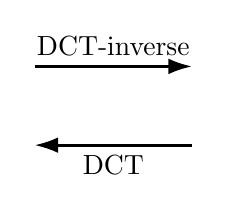
\begin{tikzpicture}
                    
                % Flèche avec étiquette
                \draw[-{Latex[length=3mm, width=2mm]}, line width=1pt] (0,1) -- (2,1) node[midway, above] {DCT-inverse};
        
                % Flèche simple
                \draw[-{Latex[length=3mm, width=2mm]}, line width=1pt] (2,0) -- (0,0) node[midway, below] {DCT};

            \end{tikzpicture}

        \end{column}
\end{comment}


\begin{frame}{Un exemple}

    \centering
    \begin{figure}
        \centering
        \includegraphics[width=0.25\linewidth]{bloc_88.png}
        \caption{une matrice 8$\times$8}
    \end{figure}

    \begin{minipage}{0.45\textwidth}
        \centering
        \begin{table}
            \tiny 
            \centering
            \setlength{\tabcolsep}{2pt} % Réduire l'espace entre les colonnes
            \renewcommand{\arraystretch}{1.25} % Ajuste l'espace entre les lignes
            \begin{tabular}{cccccccc}
                160 & 156 & 153 & 147 & 140 & 134 & 127 & 108\\
                156 & 151 & 148 & 143 & 126 & 114 & 105 & 83\\
                153 & 144 & 138 & 140 & 117 & 97 & 82 & 61\\
                142 & 141 & 142 & 149 & 116 & 95 & 67 & 68\\
                126 & 120 & 124 & 121 & 102 & 65 & 65 & 68\\
                113 & 97 & 95 & 96 & 91 & 125 & 112 & 57\\
                102 & 100 & 95 & 90 & 98 & 121 & 140 & 122\\
                106 & 104 & 106 & 92 & 98 & 121 & 142 & 139\\
            \end{tabular}
            \caption{\centering Dans la base canonique}
        \end{table}
    \end{minipage}
    \hfill
    \begin{minipage}{0.45\textwidth}
        \centering
        \begin{table}
            \tiny 
            \centering
            \setlength{\tabcolsep}{2pt} % Réduire l'espace entre les colonnes
            \renewcommand{\arraystretch}{1.25} % Ajuste l'espace entre les lignes

            \begin{tabular}{cccccccc}
                -99 & 98 & -20 & 20 & -16 & 20 & 2 & -6\\
                78 & 103 & -38 & -8 & 17 & -3 & -3 & -1\\
                58 & -75 & 40 & 0 & -13 & 1 & -8 & 13\\
                -7 & -18 & -4 & 23 & -14 & 5 & 4 & -2\\
                21 & 7 & -2 & -20 & 12 & -12 & 9 & -3\\
                12 & -10 & 1 & -2 & 2 & 0 & -6 & 0\\
                -9 & 4 & -3 & 15 & -7 & 8 & 0 & 0\\
                -2 & -2 & 6 & -5 & 5 & -7 & 2 & 1\\
            \end{tabular}
            \caption{\centering Dans la base DCT}
        \end{table}
    \end{minipage}
    \hfill
\end{frame}


\begin{frame} {Quantification}
    \begin{figure}
        \centering
        \begin{tikzpicture}
            % Inclure l'image
            \node[anchor=south west,inner sep=0] (image) at (0,0) {
                \includegraphics[width=1\linewidth, trim=0cm 25cm 0cm 0cm, clip]{Compression_JPEG.png}
            };
            % Dessiner un carré rouge
            \begin{scope}[x={(image.south east)},y={(image.north west)}]
                % Coordonnées du carré : (x, y) pour le coin inférieur gauche
                \draw[red,ultra thick] (0.735,0.02) rectangle (0.855,0.98);
            \end{scope}
        \end{tikzpicture}
        %\caption{Étapes de la compression JPEG}
    \end{figure}
\end{frame}


\begin{frame}{Quantification}
    % expliquer le principe (on divise les valeurs par cette matrice)
    \begin{minipage}{1\textwidth}
    La matrice de fréquence est divisée par la matrice de quantification.
        \begin{itemize}
            \item L'objectif est de réduire la taille de l'information en approximant les basses fréquences et en éliminant les hautes fréquences.
            \item Plus les valeurs de quantification sont grandes, plus la perte est importante, mais la compression est meilleure.
            \item \textbf{\Large k} est le facteur de quantification.
        \end{itemize}        
    \end{minipage}
    \hfill
    
    \vspace{17pt}

    \tiny 
    \begin{minipage}{0.29\textwidth}
        \centering
        \begin{table}
            \tiny 
            \centering
            \setlength{\tabcolsep}{2pt} % Réduire l'espace entre les colonnes
            \renewcommand{\arraystretch}{1.2} % Ajuste l'espace entre les lignes

            \begin{tabular}{cccccccc}
                -99 & 98 & -20 & 20 & -16 & 20 & 2 & -6\\
                78 & 103 & -38 & -8 & 17 & -3 & -3 & -1\\
                58 & -75 & 40 & 0 & -13 & 1 & -8 & 13\\
                -7 & -18 & -4 & 23 & -14 & 5 & 4 & -2\\
                21 & 7 & -2 & -20 & 12 & -12 & 9 & -3\\
                12 & -10 & 1 & -2 & 2 & 0 & -6 & 0\\
                -9 & 4 & -3 & 15 & -7 & 8 & 0 & 0\\
                -2 & -2 & 6 & -5 & 5 & -7 & 2 & 1\\
            \end{tabular}
            \caption*{\centering \tiny  matrice après DCT \\ \ }
        \end{table}
    \end{minipage}
    \hfill
    \begin{minipage}{0.09\textwidth}
        \centering
        \Large
        \vspace{-40pt}
        $ \textbf{ \textbf{\tiny \ }k $\div$} $
    \end{minipage}
    \hfill
    \begin{minipage}{0.3\textwidth}
        \centering
        \begin{table}
            \tiny 
            \centering
            \setlength{\tabcolsep}{2pt} % Réduire l'espace entre les colonnes
            \renewcommand{\arraystretch}{1.2} % Ajuste l'espace entre les lignes
            \begin{tabular}{cccccccc}
                16 & 11 & 10 & 16 & 24 & 40 & 51 & 61\\
                12 & 12 & 14 & 19 & 26 & 58 & 60 & 55\\
                14 & 13 & 16 & 24 & 40 & 57 & 69 & 56\\
                14 & 17 & 22 & 29 & 51 & 87 & 80 & 62\\
                18 & 22 & 37 & 56 & 68 & 109 & 103 & 77\\
                24 & 35 & 55 & 64 & 81 & 104 & 113 & 92\\
                49 & 64 & 78 & 87 & 103 & 121 & 120 & 101\\
                72 & 92 & 95 & 98 & 112 & 100 & 103 & 99\\
            \end{tabular}
            \caption*{\centering \tiny matrice de quantification choisie empiriquement par JPEG}
        \end{table}
    \end{minipage}
    \hfill
    \begin{minipage}{0.03\textwidth}
        \centering
        \Large
        \vspace{-40pt}
        $ \ \textbf{=} $
    \end{minipage}
    \hfill
    \begin{minipage}{0.23\textwidth}
        \centering
        \begin{table}
            \tiny 
            \centering
            \setlength{\tabcolsep}{2pt} % Réduire l'espace entre les colonnes
            \renewcommand{\arraystretch}{1.2} % Ajuste l'espace entre les lignes
            \begin{tabular}{cccccccc}
                -6 & 9 & -2 & 1 & -1 & 0 & 0 & 0 \\
                6 & 9 & -3 & 0 & 1 & 0 & 0 & 0 \\
                4 & -6 & 2 & 0 & 0 & 0 & 0 & 0 \\
                0 & -1 & 0 & 1 & 0 & 0 & 0 & 0 \\
                1 & 0 & 0 & 0 & 0 & 0 & 0 & 0 \\
                0 & 0 & 0 & 0 & 0 & 0 & 0 & 0 \\
                0 & 0 & 0 & 0 & 0 & 0 & 0 & 0 \\
                0 & 0 & 0 & 0 & 0 & 0 & 0 & 0 \\
            \end{tabular}
            \caption*{\centering \tiny Matrice quantifiée \\ \ }
        \end{table}
    \end{minipage}

\end{frame}

\begin{comment}

\begin{frame} {Sur la matrice de quantification}
    \centering
    Les hautes fréquences sont davantage approximées que les basses fréquences.
    
    \vspace{15pt}
    \begin{table}
        \tiny 
        \centering
        \renewcommand{\arraystretch}{1.1} % Ajuste l'espace entre les lignes

        \setlength{\tabcolsep}{2pt} % Réduire l'espace entre les colonnes
        \begin{tabular}{cccccccc}
            16 & 11 & 10 & 16 & 24 & 40 & 51 & 61\\
            12 & 12 & 14 & 19 & 26 & 58 & 60 & 55\\
            14 & 13 & 16 & 24 & 40 & 57 & 69 & 56\\
            14 & 17 & 22 & 29 & 51 & 87 & 80 & 62\\
            18 & 22 & 37 & 56 & 68 & 109 & 103 & 77\\
            24 & 35 & 55 & 64 & 81 & 104 & 113 & 92\\
            49 & 64 & 78 & 87 & 103 & 121 & 120 & 101\\
            72 & 92 & 95 & 98 & 112 & 100 & 103 & 99\\
        \end{tabular}
        \caption{\centering matrice de quantification choisie empiriquement par JPEG} %Quantification commune pour la luminance
    \end{table}
\end{frame}

\end{comment}

\begin{frame} {Codage entropique}
    \begin{figure}
        \centering
        \begin{tikzpicture}
            % Inclure l'image
            \node[anchor=south west,inner sep=0] (image) at (0,0) {
                \includegraphics[width=1\linewidth, trim=0cm 25cm 0cm 0cm, clip]{Compression_JPEG.png}
            };
            % Dessiner un carré rouge
            \begin{scope}[x={(image.south east)},y={(image.north west)}]
                % Coordonnées du carré : (x, y) pour le coin inférieur gauche
                \draw[red,ultra thick] (0.88,0.02) rectangle (0.998,0.98);
            \end{scope}
        \end{tikzpicture}
        %\caption{Étapes de la compression JPEG}
    \end{figure}
\end{frame}

\begin{frame} {Parcours en zigzag}
    \hfill
    \begin{minipage}{0.35\textwidth}
        \centering
        \begin{figure}
            \centering
            \includegraphics[width=0.9\linewidth]{zigzag2.png}
            \caption{\centering Parcours en zigzag}
        \end{figure}
    \end{minipage}
    \hfill
    \begin{minipage}{0.05\textwidth}
    \end{minipage}
    \hfill
    \begin{minipage}{0.45\textwidth}
        \centering
        \begin{table}
            \tiny 
            \centering
            \setlength{\tabcolsep}{2pt} % Réduire l'espace entre les colonnes
            \renewcommand{\arraystretch}{1.25} % Ajuste l'espace entre les lignes
            \begin{tabular}{cccccccc}
                -6 & 9 & -2 & 1 & -1 & 0 & 0 & 0 \\
                6 & 9 & -3 & 0 & 1 & 0 & 0 & 0 \\
                4 & -6 & 2 & 0 & 0 & 0 & 0 & 0 \\
                0 & -1 & 0 & 1 & 0 & 0 & 0 & 0 \\
                1 & 0 & 0 & 0 & 0 & 0 & 0 & 0 \\
                0 & 0 & 0 & 0 & 0 & 0 & 0 & 0 \\
                0 & 0 & 0 & 0 & 0 & 0 & 0 & 0 \\
                0 & 0 & 0 & 0 & 0 & 0 & 0 & 0 \\
            \end{tabular}
            \caption{\centering Matrice après quantification }
        \end{table}
        
        \vspace{10pt} 

        \scriptsize
        \centering
        Après zigzag : \\ -6, 9, 6, 4, 9, -2, 1, -3, -6, 0, 1, -1, 2, 0, -1, 0, 1, 0, 0, 0, 0, 0, 0, 0, 1, EOB \\
    \end{minipage}


\end{frame}


\begin{frame} {Codage entropique}

    \hfill
    \begin{minipage}{0.5\textwidth}
        \scriptsize

        Pour le codage RLE on code chaque \\ coefficient non nul sous la forme :\\
        ( 0-tête / catégorie ) [position]
        \begin{itemize}
            \item 0-tête : nombre des zéros qui le séparent de son prédecesseur non-nul 
            \item catégorie : catégorie du coefficient
            \item position : position dans la catégorie
        \end{itemize}
    \end{minipage}
    \hfill
    \begin{minipage}{0.43\textwidth}
        \begin{figure}
            \centering
            \includegraphics[width=1\linewidth]{table_codage_entropique.png}
            \caption{Table des catégories}
        \end{figure}
    \end{minipage}
    \hfill

    \vspace{20pt} 
    
    \scriptsize
    \centering
    
    Après zigzag : -6, 9, 6, 4, 9, -2, 1, -3, -6, 0, 1, -1, 2, 0, -1, 0, 1, 0, 0, 0, 0, 0, 0, 0, 1, EOB \\ \ \\
    après codage RLE : (0,3) 1, (0,4) 9, (0,3) 6, (0,3) 4, (0,4) 9, (0,2) 1, (0,1) 1, (0,2) 0, (0,3) 1, (1,1) 1, (0,1) 0, (0,2) 2, (1,1) 0, (1,1) 1, (7,1) 1, (0,0) \\ \ \\
    après Huffman : 100 001 1011 1001 100 110 100 100 1011 1001 01 01 00 1 01 00 100 001 1100 1 00 0 01 11 1100 0 1100 1 11111010 1 1010

\end{frame}


\begin{frame} {Décompression}

    \begin{itemize}
        \item Décompression de Huffman
        \item Déduction de la liste à partir du codage RLE
        \item Reconstruction de la matrice quantifiée
        \item Multiplication par la matrice de quantification
        \item Utilisation de la DCT-inverse
        \item Assemblage des matrices 8x8
        \item Sur-échantillonnage
        \item Transformation des couleurs de YCbCr vers RVB
    \end{itemize}
\end{frame}


%------------------------------------------------
\section{Analyse des performances en taille et qualité}
%------------------------------------------------

\begin{frame}
	\sectionpage
\end{frame}

\begin{comment}

\begin{frame} {Objectif}
    % expliquer que j'ai codé la compression JPEG en python
    % Que ça va me permettre d'estimer la taille de l'image compressé
    % que je vais estimer la qualité de l'image en me basant sur la différencede couleur avec l'image originale
    % Estimation de la qualité de l’image à partir de la différence de couleur entre image originale et image compressée.
    \footnotesize
    Mon objectif est de choisir pour chaque image le niveau de compression à appliquer.
    Je souhaite à la fois garantir la qualité de l'image et réduire sa taille au maximum.
    Il faut donc un moyen d'estimer la qualité d'une image
    
    
    Je souhaite estimer la taille et la qualité d'une image.
    \\ Ayant codé la compression JPEG en python je peux estimer la taille.
    \\ Objectif : estimer/quantifier la qualité d'une image
    
\end{frame}

\end{comment}

\begin{frame} {Premier indice de qualité : le PSSB}
    \centering
    \scriptsize

    
    Racine de l'Erreur Quadratique Moyenne : REQM
    \[
    \text{REQM} = \sqrt{\frac{1}{3np} \sum_{i=0}^{n-1} \sum_{j=0}^{p-1} \sum_{k=0}^{2} \left( \text{img}(i, j, k) - \text{imgd}(i, j, k) \right)^2}
    \]

    \centering
    \scriptsize
    \ \\ \ \\  Rapport du Pic du Signal Sur Bruit : PSSB
    \[
    \text{PSSB} = 20 \cdot \log_{10} \left( \frac{255}{\text{REQM}} \right)
    \]

\end{frame}

\begin{frame} {Second indice de qualité : le SSIM}
    \centering
    \scriptsize
    Structural SIMilarity : SSIM
    
    \[
        \text{SSIM} = 
        \underbrace{\frac{(2\mu_x\mu_y + c_1)}{(\mu_x^2 + \mu_y^2 + c_1)}}_{\text{\scriptsize luminance}}
        \times
        \underbrace{\frac{(2\sigma_x\sigma_y + c_2)}{(\sigma_x^2 + \sigma_y^2 + c_2)}}_{\text{\scriptsize contraste}}
        \times
        \underbrace{\frac{(\text{cov}_{xy} + c_3)}{(\sigma_x\sigma_y + c_3)}}_{\text{\scriptsize structure}}
    \]

    \[
        \text{avec} \ 
        \begin{cases}
        \text{$x$ et $y$ deux matrices} \\
        \text{$\mu_x$ la moyenne de $x$, $\mu_y$ la moyenne de $y$} \\
        \text{$\sigma_x^2$ la variance de $x$, $\sigma_y^2$ la variance de $y$} \\
        \text{$\text{cov}_{xy}$ la covariance de $x$ et $y$} \\        
        \text{$c_1 = 6.5$, $c_2 = 58.5$ et $c_3 = 29.2$} \\        
        \end{cases}
    \]

\end{frame}

\begin{frame}{Échantillon de 12 des 46 photos utilisées} 

    \hfill
    \begin{minipage}{.23\textwidth}
        \centering
        \begin{figure}
            \includegraphics[width=.75\linewidth]{photos_utilises/1.jpg}
        \end{figure}
        \begin{figure}
            \includegraphics[width=1\linewidth]{photos_utilises/2.jpg}
        \end{figure}
        \begin{figure}
            \includegraphics[width=1\linewidth]{photos_utilises/3.jpg}
        \end{figure}
    \end{minipage}
    \hfill
    \begin{minipage}{.23\textwidth}
        \centering
        \begin{figure}
            \includegraphics[width=.75\linewidth]{photos_utilises/15.jpg}
        \end{figure}
        \begin{figure}
            \includegraphics[width=1\linewidth]{photos_utilises/6.jpg}
        \end{figure}
        \begin{figure}
            \includegraphics[width=1\linewidth]{photos_utilises/12.jpg}
        \end{figure}
    \end{minipage}
    \hfill
    \begin{minipage}{.23\textwidth}
        \centering
        \begin{figure}
            \includegraphics[width=.75\linewidth]{photos_utilises/25.jpg}
        \end{figure}
        \begin{figure}
            \includegraphics[width=1\linewidth]{photos_utilises/17.jpg}
        \end{figure}
        \begin{figure}
            \includegraphics[width=1\linewidth]{photos_utilises/23.jpg}
        \end{figure}
    \end{minipage}
    \hfill
    \begin{minipage}{.23\textwidth}
        \centering
        \begin{figure}
            \includegraphics[width=.75\linewidth]{photos_utilises/35.jpg}
        \end{figure}
        \begin{figure}
            \includegraphics[width=1\linewidth]{photos_utilises/27.jpg}
        \end{figure}
        \begin{figure}
            \includegraphics[width=1\linewidth]{photos_utilises/41.jpg}
        \end{figure}
    \end{minipage}
    \hfill
    \vspace{0.1cm}
    \textit{\tiny \\ \centering source des images (CC0 1.0) : https://www.signatureedits.com/free-raw-photos/}


\end{frame}

\begin{frame} {Résultats}
    \begin{figure}
        \centering
        \includegraphics[width=1\linewidth]{graphe1.png}
    \end{figure}
    
\end{frame}

\begin{frame} {Résultats}
    \begin{figure}
        \centering
        \includegraphics[width=1\linewidth]{graphe2.png}
    \end{figure}
    
\end{frame}

\begin{frame} {Résultats}
    \centering
    \begin{figure}
        \centering
        \includegraphics[width=1\linewidth]{graphe3.png}
    \end{figure}
    
\end{frame}

\begin{frame} {Conclusion}
    \begin{itemize}
        \item Les indices de qualité permettent de comparer la qualité d'une même image.
        \item Il est facile de réduire la taille d'une image d'un facteur 10.
        \item Le meilleur facteur de quantification à choisir est 1 dans mon étude.
    \end{itemize}



\end{frame}






%----------------------------------------------------------------------------------------%----------------------------------------------------------------------------------------%----------------------------------------------------------------------------------------


\begin{frame} {Annexe}
    \Huge Annexe
\end{frame}

\begin{comment}
    
\begin{frame} {Exemple de compression décompression}
    \centering
    \hfill
    \begin{minipage}{0.28\textwidth}

        \begin{figure}
            \centering
            \includegraphics[width=1\linewidth]{mi_temps_0_10.png}
            \caption{\centering image originale}
        \end{figure}
        
        \tiny
        10011011 10011100 10010110
        10011011 10011010 10010101
        10001101 10001010 10000011
        10000110 10000010 01110110
        10001110 10001010 01111110
        10001100 10000111 01111011
        10000110 10000000 01110100
        10000100 01111110 01110011
        10010110 10001111 10000101
        10001101 10000110 01111100
        10001010 10000011 01111001
        10011010 10010101 10001010
        \textbf{...}
        
    \end{minipage}
    \hfill
    \begin{minipage}{0.28\textwidth}

         \small Image compressée :
         \vspace{.3cm} \\ 
         \ \ 
         \tiny
         \seqsplit{01100011010\ 0011010\ 0000110011000001100001010\ 010001000101001010101101111011100011111101011010\ 10011000001100000110000110010001010\ 1001101010\ 1001011010\ 1001011010\ 1001011010\ 10010011000110000011010\ 01111010\ 10010011111100001010\ 1001001010} \\ \textbf{...}

        % 1001001010\ 01111010\ 01110001010\ 01111010\ 01111010\ 01111010\ 01111010\ 01111010\ 01111010\ 01101010\ 01101010\ 01101010\ 01101010\ 01101010\ 01101010\ 01101010\ 01101010\ 01101010\ 01101010\ 01101010\ 1101110010101010101111101111010\ 10001100101110110011111101000011010\ 01000101111101010011110011010\ 1110000000000001010\ 01000100001001001100101001000111101101010\ 01110001010\ 0110000111110111100010011100111101101010\ 011011111111100101101000011111101001010


        
    \end{minipage}
    \hfill
    \begin{minipage}{0.28\textwidth}
        \begin{figure}
            \centering
            \includegraphics[width=1\linewidth]{mi_temps_8_0.16.png}
            \caption{\centering image décompressée}
        \end{figure}
        \tiny
        10011000 10011000 10011000
        10010110 10010110 10010110
        10010011 10010011 10010011
        10001110 10001110 10001110
        10001010 10001010 10001010
        10000101 10000101 10000101
        10000010 10000010 10000010
        10000000 10000000 10000000
        10001101 10001101 10001101
        10001101 10001101 10001101
        10001101 10001101 10001101
        10001101 10001101 10001101
        \textbf{...}
    \end{minipage}
    \hfill


\end{frame}
\end{comment}


\begin{frame}{Annexe : formalisation du sous-échantillonnage de la chrominance}
    \scriptsize
    \vspace{-0.3cm}
    \[
        \textbf{J:a:b} \ 
        \begin{cases}
        \text{\textbf{J} = nombre d'échantillons de luminance Y par ligne} \\
        \text{\textbf{a} = nombre d'échantillons de chrominance (Cb, Cr) sur la première ligne} \\
        \text{\textbf{b} = nombre d'échantillons de chrominance (Cb, Cr) sur la deuxième ligne} \\        
        \end{cases}
    \]

    \vspace{0.3cm}

    \noindent
    % premier tableau en haut
    \begin{minipage}[t]{0.25\textwidth}
        \centering
        \small
      \textbf{4:4:4}
      \text{\tiny on garde toute l'information}
    \end{minipage}
    \hfill
    \begin{minipage}[t]{0.7\textwidth}
      \begin{tabular}{|c|c|c|c|}
        \hline
        1 & 2 & 3 & 4 \\
        \hline
        5 & 6 & 7 & 8 \\
        \hline
      \end{tabular}
        $ \rightarrow $
      \begin{tabular}{|c|c|c|c|}
        \hline
        1 & 2 & 3 & 4 \\
        \hline
        5 & 6 & 7 & 8 \\
        \hline
      \end{tabular}
    \end{minipage}
    
    \vspace{.6cm} % Espace entre les tableaux
    
    
    % deuxieme tableau au milieu
    \begin{minipage}[t]{0.25\textwidth}
        \centering
        \small
        \textbf{4:2:2}
        \tiny
        \shortstack{\\on garde 1 information \\ pour 2 pixels}
    \end{minipage}
    \hfill
    \begin{minipage}[t]{0.7\textwidth}
      \begin{tabular}{|c|c|c|c|}
        \hline
        1 & 2 & 3 & 4 \\
        \hline
        5 & 6 & 7 & 8 \\
        \hline
      \end{tabular}
        $ \rightarrow $
      \begin{tabular}{|c|c|}
        \hline
        1.5 & 3.5 \\
        \hline
        5.5 & 7.5 \\
        %1.5 & 1.5 & 3.5 & 3.5 \\
        %\hline
        %5.5 & 5.5 & 7.5 & 7.5 \\
        \hline
      \end{tabular}
    \end{minipage}
    
    \vspace{.6cm} % Espace entre les tableaux
    
    
    % Troisième tableau en bas
    \begin{minipage}[t]{0.25\textwidth}
        \centering
        \small
        \textbf{4:2:0}
        \tiny
        \shortstack{\\on garde 1 information \\ pour 4 pixels}
    \end{minipage}
    \hfill
    \begin{minipage}[t]{0.7\textwidth}
      \begin{tabular}{|c|c|c|c|}
        \hline
        1 & 2 & 3 & 4 \\
        \hline
        5 & 6 & 7 & 8 \\
        \hline
      \end{tabular}
        $ \rightarrow $
      \begin{tabular}{|c|c|}
        \hline
        3.5 & 5.5 \\
        \hline
      \end{tabular}
    \end{minipage}
    
\end{frame}

\begin{frame} {Annexe : la transformée de fourrier discrète}
    \centering
    Transformation de Fourier discrète
    \[
        S(k) = \sum_{n=0}^{N-1} s(n) e^{-2i\pi k \frac{n}{N}}
    \]
    Transformation de Fourier discrète inverse
    \[
        s(n) = \frac{1}{N} \sum_{k=0}^{N-1} S(k) e^{2i\pi n \frac{k}{N}}
    \]

    Transformation de Fourier discrète bidimensionnelle
    \[
        S(u, v) = \sum_{m=0}^{M-1} \sum_{n=0}^{N-1} s(m, n) e^{-2i\pi \left( \frac{um}{M} + \frac{vn}{N} \right)}        
    \]
    
\end{frame}

\begin{frame} {Annexe : comparaison entre TFD et DCT}

    \footnotesize
    \centering
    
    Transformation de Fourier discrète
    \[
        S(k) = \sum_{n=0}^{N-1} s(n) e^{-2i\pi k \frac{n}{N}} = \sum_{n=0}^{N-1} s(n) \cos\left(2\pi k \frac{n}{N}\right) - i \sum_{n=0}^{N-1} s(n) \sin\left(2\pi k \frac{n}{N}\right)

    \]

    DCT
    \begin{equation*}
        S(k) = \sum_{n=0}^{N-1} s(n) \cos \left( \frac{k\pi}{N} \left( n + \frac{1}{2} \right) \right)
    \end{equation*}    


\end{frame}


\begin{frame} {Annexe : comparaison entre TFD et DCT bidimensionnelle}

    \scriptsize
    \centering
    
    Transformation de Fourier discrète bidimensionnelle
    \[
        S(u, v) = \sum_{m=0}^{M-1} \sum_{n=0}^{N-1} s(m, n) e^{-2i\pi \left( \frac{um}{M} + \frac{vn}{N} \right)} 
    \]
    \[
        =  \sum_{m=0}^{M-1} \sum_{n=0}^{N-1} s(m, n) \cos\left(2\pi \frac{um}{M}\right)\cos\left(2\pi \frac{vn}{N}\right)
    \]  
    \[
        - \sum_{m=0}^{M-1} \sum_{n=0}^{N-1} s(m, n) \sin\left(2\pi \frac{um}{M}\right)\sin\left(2\pi \frac{vn}{N}\right)
    \]  
    \[
        - i \sum_{m=0}^{M-1} \sum_{n=0}^{N-1} s(m, n) \sin\left(2\pi \left( \frac{um}{M} + \frac{vn}{N} \right)\right) 
    \]  
    \\
    DCT
    \[
    S(u, v) = \frac{2}{N} \sum_{m=0}^{N-1} \sum_{n=0}^{N-1} s(m, n) \cos \left( \frac{\pi}{N} u \left( m + \frac{1}{2} \right) \right) \cos \left( \frac{\pi}{N} v \left( n + \frac{1}{2} \right) \right)
    \]

\end{frame}


\begin{frame}{Annexe : DCT inverse}        
    \scriptsize
    \centering
    DCT bidimensionnelle
    
    \[
    DCT(i,j) = \frac{2}{N} c(i) c(j) \sum_{x=0}^{N-1} \sum_{y=0}^{N-1} pixel(x,y) \cos \left( \frac{\pi}{N} i \left( x + \frac{1}{2} \right) \right) \cos \left( \frac{\pi}{N} j \left( y + \frac{1}{2} \right) \right)
    \]
    \[
        \text{avec} \ \ \ \ c(\alpha) =
        \begin{cases}
        \frac{1}{\sqrt{2}} & \text{si } \alpha = 0 \\
        1 & \text{sinon}
        \end{cases}
    \]
    
    \vspace{1cm} % Espace entre les tableaux

    DCT bidimensionnelle inverse
    
    \[
        pixel(x,y) = \frac{2}{N} \sum_{i=0}^{N-1} \sum_{j=0}^{N-1} c(i) c(j) DCT(i,j) \cos \left( \frac{\pi}{N} i \left( x + \frac{1}{2} \right) \right) \cos \left( \frac{\pi}{N} j \left( y + \frac{1}{2} \right) \right)
    \]
\end{frame}

\begin{frame} {Annexe : compression de Huffman}
    \footnotesize
    texte à encoder : "\textbf{le tipe valorise la curiosite}"
    \\ \ \\
    Comptage du nombre d'occurrences : [(u, 1), (v, 1), (c, 1), (p, 1), (a, 2), (o, 2), (r, 2), (s, 2), (t, 3), (l, 3), (e, 4), (i, 4), (\_, 4)]

    \begin{figure}
        \centering
        \includegraphics[width=0.5\linewidth]{compressionhuffman.png}
        \caption{Arbre de Huffman}
        \tiny \textit{source de l'image : http://lwh.free.fr/pages/algo/compression/huffman.html}
    \end{figure}

    résultat : 001 101 111 000 110 01011 101 111 01001 0110 001 0111 1000 110 1001 101 111 001 0110 111 01010 01000 1000 110 0111 1001 110 000 101

\end{frame}

\begin{frame}{Annexe : extrait de la table de Huffman} 

    \hfill
    \begin{minipage}{.49\textwidth}
        \centering
        \begin{figure}
            \includegraphics[width=.7\linewidth]{huffman1.png}
        \end{figure}
    \end{minipage}
    \hfill
    \begin{minipage}{.49\textwidth}
        \centering
        \begin{figure}
            \includegraphics[width=.7\linewidth]{huffman2.png}
        \end{figure}
    \end{minipage}
    \hfill
    \centering
    \scriptsize
    source : https://www.w3.org/Graphics/JPEG/itu-t81.pdf
\end{frame}



\begin{frame}{Annexe : SSIM}
    \scriptsize
    \textbf{Origine du SSIM :}
    \begin{itemize}
        \item \textbf{Créateurs :} Zhou Wang, Alan C. Bovik, Hamid R. Sheikh, Eero P. Simoncelli
        \item \textbf{Année :} 2004
        \item \textbf{Article :} \\
        \textit{“Image Quality Assessment: From Error Visibility to Structural Similarity”} \\
         \ IEEE Transactions on Image Processing, vol. 13, no. 4, Apr. 2004
    \end{itemize}

    \vspace{0.7cm}
    L'objectif est de remplacer les métriques traditionnelles comme le PSSB qui sont peu corrélées à la perception visuelle.
    
    \vspace{0.4cm}
    \begin{block}{}
    L'œil humain est particulièrement sensible à la \textbf{structure}, au \textbf{contraste} et à la \textbf{luminance}, plutôt qu'aux erreurs locales en intensité.
    \end{block}

    \[
        \text{SSIM} = 
        \underbrace{\frac{(2\mu_x\mu_y + c_1)}{(\mu_x^2 + \mu_y^2 + c_1)}}_{\text{luminance}}
        \times
        \underbrace{\frac{(2\sigma_x\sigma_y + c_2)}{(\sigma_x^2 + \sigma_y^2 + c_2)}}_{\text{contraste}}
        \times
        \underbrace{\frac{(\text{cov}_{xy} + c_3)}{(\sigma_x\sigma_y + c_3)}}_{\text{structure}}
    \]

\end{frame}



\begin{frame} {Annexe : SSIM}

    \[
    \text{SSIM} = \frac{(2\mu_x\mu_y + c_1)}{(\mu_x^2 + \mu_y^2 + c_1)}\frac{(2\sigma_x\sigma_y + c_2)}{(\sigma_x^2 + \sigma_y^2 + c_2)}\frac{(\text{cov}_{xy} + c_3)}{(\sigma_x\sigma_y + c_3)}
    \]
    \\ \ \\

    \begin{itemize}
        \item $c_1 = (k_1 L)^2$, $c_2 = (k_2 L)^2$ et $c_3 = \frac{c_2}{2}$ : pour stabiliser la division quand le dénominateur est très faible.
        \item $L$ : la dynamique des valeurs des pixels (255).
        \item $k_1 = 0,01$ et $k_2 = 0,03$ : des petites valeurs.
    \end{itemize}
\end{frame}

\begin{frame} {Annexe : transformation YCbCr RVB}
    \scriptsize
    \begin{align*}
        Y &= 0,299 \, R + 0,587 \, V + 0,114 \, B \\
        Cb &= -0,1687 \, R - 0,3313 \, V + 0,5 \, B + 128 \\
        Cr &= 0,5 \, R - 0,4187 \, V - 0,0813 \, B + 128
    \end{align*}
    
    \vspace{0.4cm}

    \footnotesize
    \begin{itemize}
        \item Les coefficients ont été défini en 1982 par la norme ITU-R BT.601 de l'Union Internationale des Télécommunications (ITU).
        \item Les coefficients sont basés sur la sensibilité de l'œil aux couleurs.
        \item La luminance est l'intensité lumineuse perçue par l'œil qui est très sensible au vert, un peu moins au rouge, et beaucoup moins au bleu.
    \end{itemize}

    
    \vspace{0.7cm}
    
    Les composantes \textbf{Cb} et \textbf{Cr} approximent $B - Y$ et $R - Y$ (différences de couleur).
    
    \begin{itemize}
        \item \textbf{Cb} : axe \textcolor{blue}{bleu} $\leftrightarrow$ \textcolor{orange}{jaune}
        \item \textbf{Cr} : axe \textcolor{red}{rouge} $\leftrightarrow$ \textcolor{cyan}{cyan}
    \end{itemize}
    
    \vspace{0.4cm}
\end{frame}


\begin{frame} {Annexe : différentes matrices de quantification}
    \begin{minipage}{0.3\textwidth}
        \centering
        \begin{table}
        \tiny 
        \centering
        \renewcommand{\arraystretch}{1.1} % Ajuste l'espace entre les lignes

        \setlength{\tabcolsep}{2pt} % Réduire l'espace entre les colonnes
            \begin{tabular}{cccccccc}
                3 & 3 & 3 & 3 & 3 & 3 & 3 & 3\\
                3 & 3 & 3 & 3 & 3 & 3 & 3 & 3\\
                3 & 3 & 3 & 3 & 3 & 3 & 3 & 3\\
                3 & 3 & 3 & 3 & 3 & 3 & 3 & 3\\
                3 & 3 & 3 & 3 & 3 & 3 & 3 & 3\\
                3 & 3 & 3 & 3 & 3 & 3 & 3 & 3\\
                3 & 3 & 3 & 3 & 3 & 3 & 3 & 3\\
                3 & 3 & 3 & 3 & 3 & 3 & 3 & 3\\
            \end{tabular}
            \caption{\centering Quantification constante $Q_i_j = K$ \\ (ici $K = 3$)}
        \end{table}
    \end{minipage}
    \hfill
    \begin{minipage}{0.3\textwidth}
        \centering
        \begin{table}
            \tiny 
            \renewcommand{\arraystretch}{1.1} % Ajuste l'espace entre les lignes
            \centering
            \setlength{\tabcolsep}{2pt} % Réduire l'espace entre les colonnes
    
                  \begin{tabular}{cccccccc}
                3 & 5 & 7 & 9 & 11 & 13 & 15 & 17\\
                5 & 7 & 9 & 11 & 13 & 15 & 17 & 19\\
                7 & 9 & 11 & 13 & 15 & 17 & 19 & 21\\
                9 & 11 & 13 & 15 & 17 & 19 & 21 & 23\\
                11 & 13 & 15 & 17 & 19 & 21 & 23 & 25\\
                13 & 15 & 17 & 19 & 21 & 23 & 25 & 27\\
                15 & 17 & 19 & 21 & 23 & 25 & 27 & 29\\
                17 & 19 & 21 & 23 & 25 & 27 & 29 & 31\\
            \end{tabular}
            \caption{\centering Quantification $Q_i_j = 1 + K(1 + i + j)$ \\ (ici $K = 2$)}
        \end{table}
    \end{minipage}
    \hfill
    \begin{minipage}{0.3\textwidth}
        \centering
        \begin{table}
            \tiny 
            \centering
            \renewcommand{\arraystretch}{1.1} % Ajuste l'espace entre les lignes
    
            \setlength{\tabcolsep}{2pt} % Réduire l'espace entre les colonnes
            \begin{tabular}{cccccccc}
                16 & 11 & 10 & 16 & 24 & 40 & 51 & 61\\
                12 & 12 & 14 & 19 & 26 & 58 & 60 & 55\\
                14 & 13 & 16 & 24 & 40 & 57 & 69 & 56\\
                14 & 17 & 22 & 29 & 51 & 87 & 80 & 62\\
                18 & 22 & 37 & 56 & 68 & 109 & 103 & 77\\
                24 & 35 & 55 & 64 & 81 & 104 & 113 & 92\\
                49 & 64 & 78 & 87 & 103 & 121 & 120 & 101\\
                72 & 92 & 95 & 98 & 112 & 100 & 103 & 99\\
            \end{tabular}
            \caption{\centering matrice de quantification choisie empiriquement par JPEG} %Quantification commune pour la luminance
        \end{table}
    \end{minipage}
    \hfill

\end{frame}


\begin{frame} {Annexe : inconvénients de JPEG}
    \footnotesize
    \begin{itemize}
        \item Apparition de blocs de 8×8 pixels : effet de mosaïque.
        \item Des dégradés avec paliers sont visibles.
        \item Non adapté pour les dessins, les textes ou les logos car les artefacts y sont fortement visibles (en raison des contrastes important).
        \item Non adapté pour les modifications successives, la retouche photo n'est pas possible. 
    \end{itemize}
    
    \vspace{1cm}

    JPEG2000 règle ces problèmes avec l'utilisation d'ondelettes.
\end{frame}


\begin{frame}[fragile]{Code python : imports et variable globale }
    \begin{lstlisting}[style=pythonStyle]
# Les modules utilisés
from random import randrange 
import numpy as np
import math
import cv2 as cv
import matplotlib.pyplot as plt
import statistics
import copy
import os

bit_dict = {
    "0/0": "1010", "0/1": "00", "0/2": "01", "0/3": "100", "0/4": "1011", "0/5": "11010", "0/6": "1111000", "0/7": "11111000", "0/8": "1111110110", "0/9": "1111111110000010", "0/A": "1111111110000011",
    "1/1": "1100", "1/2": "11011", "1/3": "1111001", "1/4": "111110110", "1/5": "11111110110", "1/6": "1111111110000100", "1/7": "1111111110000101", "1/8": "1111111110000110", "1/9": "1111111110000111", "1/A": "1111111110001000",
    "2/1": "11100", "2/2": "11111001", "2/3": "1111110111", "2/4": "111111110100", "2/5": "1111111110001001", "2/6": "1111111110001010", "2/7": "1111111110001011", "2/8": "1111111110001100", "2/9": "1111111110001101", "2/A": "1111111110001110",
    ...
    # dictionnaire trop long pour tout afficher
    ...
    "F/0": "11111111001", "F/1": "1111111111110101", "F/2": "1111111111110110", "F/3": "1111111111110111", "F/4": "1111111111111000", "F/5": "1111111111111001", "F/6": "1111111111111010", "F/7": "1111111111111011", "F/8": "1111111111111100", "F/9": "1111111111111101", "F/A": "1111111111111110",
}
    \end{lstlisting}
\end{frame}

\begin{frame}[fragile]{Code python : rvb to ycbcr}
    \begin{lstlisting}[style=pythonStyle]
def rvb_to_ycbcr(img):
    """ renvoie 3 nouvelles matrices contenant les valeur Y Cb Cr """
    hauteur = len(img)
    largeur = len(img[0])
    mat_y = [[0 for _ in range(largeur)] for _ in range(hauteur)]
    mat_cb = [[0 for _ in range(largeur)] for _ in range(hauteur)]
    mat_cr = [[0 for _ in range(largeur)] for _ in range(hauteur)]
    for i in range(0, hauteur):
        for j in range(0, largeur):
            mat_y[i][j] = round(0.299 * img[i][j][0] + 0.587 * img[i][j][1] + 0.114 * img[i][j][2])
            mat_cb[i][j] = round(-0.1687 * img[i][j][0] - 0.3313 * img[i][j][1] + 0.5 * img[i][j][2] + 128)
            mat_cr[i][j] = round(0.5 * img[i][j][0] - 0.4187 * img[i][j][1] - 0.0813 * img[i][j][2] + 128)
    return mat_y, mat_cb, mat_cr
    \end{lstlisting}
\end{frame}

\begin{frame}[fragile]{Code python : YCbCr to RVB}
    \begin{lstlisting}[style=pythonStyle]
def ycbcr_to_rvb(mat_y, mat_cb, mat_cr):
    """ renvoie l'image en RVB """
    hauteur = len(mat_y)
    largeur = len(mat_y[0])
    img = [[[0, 0, 0] for _ in range(largeur)] for _ in range(hauteur)]
    for i in range(0, hauteur):
        for j in range(0, largeur):
            img[i][j] = [round(mat_y[i][j] + 1.402 * (mat_cr[i][j] - 128)),
                         round(mat_y[i][j] - 0.34414 * (mat_cb[i][j] - 128) - 0.71414 * (mat_cr[i][j] - 128)),
                         round(mat_y[i][j] + 1.772 * (mat_cb[i][j] - 128))]
            for k in range(0, 3):
                if img[i][j][k] < 0:
                    img[i][j][k] = 0
                elif img[i][j][k] > 255:
                    img[i][j][k] = 255
    return img
    \end{lstlisting}
\end{frame}

\begin{frame}[fragile]{Code python : sous échantillonnage 420}
    \begin{lstlisting}[style=pythonStyle]
def sous_echantillonnage_420(img):
    """renvoie une matrice sous-échantillonnée en 420"""
    res_hauteur = int(len(img) / 2)
    res_largeur = int(len(img[0]) / 2)
    res = [[0 for _ in range(res_largeur)] for _ in range(res_hauteur)]
    for i in range(0, res_hauteur):
        for j in range(0, res_largeur):
            res[i][j] = round(
                (img[2 * i][2 * j] + img[2 * i][2 * j + 1] + img[2 * i + 1][2 * j] + img[2 * i + 1][2 * j + 1]) / 4)
    return res


def sous_echantillonnage_420_inverse(mat, hauteur, largeur):
    """renvoie une matrice sur-échantillonnée en 420 de taille hauteur x largeur"""
    mat_res = [[0 for _ in range(largeur)] for _ in range(hauteur)]
    for i in range(0, hauteur):
        for j in range(0, largeur):
            mat_res[i][j] = mat[int(i / 2)][int(j / 2)]
    return mat_res
    \end{lstlisting}
\end{frame}

\begin{frame}[fragile]{Code python : sous échantillonnage 422}
    \begin{lstlisting}[style=pythonStyle]
def sous_echantillonnage_422(img):
    """renvoie une matrice sous-échantillonnée en 422"""
    res_hauteur = len(img)
    res_largeur = int(len(img[0]) / 2)
    res = [[0 for _ in range(res_largeur)] for _ in range(res_hauteur)]

    for i in range(0, res_hauteur):
        for j in range(0, res_largeur):
            res[i][j] = round((img[i][2 * j] + img[i][2 * j + 1]) / 2)
    return res


def sous_echantillonnage_422_inverse(mat, hauteur, largeur):
    """renvoie une matrice sur-échantillonnée en 422 de taille hauteur x largeur"""
    mat_res = [[0 for _ in range(largeur)] for _ in range(hauteur)]
    for i in range(0, hauteur):
        for j in range(0, largeur):
            mat_res[i][j] = mat[i][int(j / 2)]
    return mat_res
    \end{lstlisting}
\end{frame}

\begin{frame}[fragile]{Code python : trois fonctions utiles}
    \begin{lstlisting}[style=pythonStyle]
def mettre_a_dimension(mat, hauteur, largeur):
    """ :param mat: une matrice
    :param hauteur: entier inférieur à la hauteur de la matrice
    :param largeur: entier inférieur à la largeur de la matrice
    :return: la matrice extraite en haut à gauche de taille hauteur x largeur """
    mat_res = [[0 for _ in range(largeur)] for _ in range(hauteur)]
    for i in range(0, hauteur):
        for j in range(0, largeur):
            mat_res[i][j] = mat[i][j]
    return mat_res

def une_to_trois(mat):
    """renvoie la matrice sous forme d'image en nuance de gris"""
    hauteur = len(mat)
    largeur = len(mat[0])
    new = [[[0, 0, 0] for _ in range(largeur)] for _ in range(hauteur)]
    for i in range(0, hauteur):
        for j in range(0, largeur):
            new[i][j] = [mat[i][j], mat[i][j], mat[i][j]]
    return new

def ajouter_k_chaque_pixel(mat, k):
    """ applique un ajout de k à tous les coefficients de la matrice """
    hauteur = len(mat)
    largeur = len(mat[0])
    for i in range(0, hauteur):
        for j in range(0, largeur):
            mat[i][j] = mat[i][j] + k
    \end{lstlisting}
\end{frame}

\begin{frame}[fragile]{Code python : la DCT}
    \begin{lstlisting}[style=pythonStyle]
def dct_bidimensionnelle(mat):
    """ renvoie la dct d'une matrice 8x8 avec la méthode naïve"""
    res = [[0 for _ in range(8)] for _ in range(8)]
    c = [math.sqrt(2) / 2, 1, 1, 1, 1, 1, 1, 1]
    for i in range(0, 8):
        for j in range(0, 8):
            somme = 0
            for x in range(0, 8):
                for y in range(0, 8):
                    somme = somme + mat[x][y] * math.cos(((2 * x + 1) * math.pi * i) / 16) * math.cos(
                        ((2 * y + 1) * math.pi * j) / 16)
            res[i][j] = 0.25 * c[i] * c[j] * somme
    return res

def dct_bidimensionnelle_inverse(mat_dct):
    """ renvoie la dct inverse à une matrice 8x8 avec la méthode naïve"""
    pixel = [[0 for _ in range(8)] for _ in range(8)]
    c = [math.sqrt(2) / 2, 1, 1, 1, 1, 1, 1, 1]
    for x in range(0, 8):
        for y in range(0, 8):
            somme = 0
            for i in range(0, 8):
                for j in range(0, 8):
                    somme = somme + c[i] * c[j] * mat_dct[i][j] * math.cos(((2 * x + 1) * math.pi * i) / 16) * math.cos(
                        ((2 * y + 1) * math.pi * j) / 16)
            pixel[x][y] = round(0.25 * somme)
    return pixel
    \end{lstlisting}
\end{frame}

\begin{frame}[fragile]{Code python : des quantifications}
    \begin{lstlisting}[style=pythonStyle]
def quantification_constante(mat_dct, k):
    """ divise toutes les valeurs d'une matrice 8x8 par k"""
    for i in range(0, 8):
        for j in range(0, 8):
            mat_dct[i][j] = int(mat_dct[i][j] / k)


def quantification_croissante(mat_dct, k):
    """ divise toutes les valeurs d'une matrice 8x8 par 1 + k * (1+i+j)"""
    for i in range(0, 8):
        for j in range(0, 8):
            mat_dct[i][j] = int(mat_dct[i][j] / (1 + k * (1 + i + j)))


def quantification_croissante_inverse(mat_dct, k):
    """ multiplie toutes les valeurs d'une matrice 8x8 par 1 + k * (1+i+j)"""
    for i in range(0, 8):
        for j in range(0, 8):
            mat_dct[i][j] = mat_dct[i][j] * (1 + k * (1 + i + j))

    \end{lstlisting}
\end{frame}

\begin{frame}[fragile]{Code python : la quantification fournie par JPEG}
    \begin{lstlisting}[style=pythonStyle]
mat_q_commune = [
    [16, 11, 10, 16, 24, 40, 51, 61],
    [12, 12, 14, 19, 26, 58, 60, 55],
    [14, 13, 16, 24, 40, 57, 69, 56],
    [14, 17, 22, 29, 51, 87, 80, 62],
    [18, 22, 37, 56, 68, 109, 103, 77],
    [24, 35, 55, 64, 81, 104, 113, 92],
    [49, 64, 78, 87, 103, 121, 120, 101],
    [72, 92, 95, 98, 112, 100, 103, 99]
]

def quantification_originale(mat_dct, k):
    """ applique la quantification avec la matrice établie empiriquement par JPEG"""
    for i in range(0, 8):
        for j in range(0, 8):
            mat_dct[i][j] = round((mat_dct[i][j] * k) / (mat_q_commune[i][j]))

def quantification_originale_inverse(mat_dct, k):
    """ applique la quantification inverse avec la matrice établie empiriquement par JPEG"""
    for i in range(0, 8):
        for j in range(0, 8):
            mat_dct[i][j] = (mat_dct[i][j] * mat_q_commune[i][j]) / k

    \end{lstlisting}
\end{frame}

\begin{frame}[fragile]{Code python : parcours en zig zag}
    \begin{lstlisting}[style=pythonStyle]
def codage_zig_zag(mat):
    """ renvoie la liste du parcours en zig zag d'une matrice 8x8 """
    res = [mat[0][0], mat[0][1], mat[1][1], mat[2][0], mat[1][1], mat[0][2], mat[0][3], mat[1][2],
           mat[2][1], mat[3][0], mat[4][0], mat[3][1], mat[2][2], mat[1][3], mat[0][4], mat[0][5],
           mat[1][4], mat[2][3], mat[3][2], mat[4][1], mat[5][0], mat[6][0], mat[5][1], mat[4][2],
           mat[3][3], mat[2][4], mat[1][5], mat[0][6], mat[0][7], mat[1][6], mat[2][5], mat[3][4],
           mat[4][3], mat[5][2], mat[6][1], mat[7][0], mat[7][1], mat[6][2], mat[5][3], mat[4][4],
           mat[3][5], mat[2][6], mat[1][7], mat[2][7], mat[3][6], mat[4][5], mat[5][4], mat[6][3],
           mat[7][2], mat[7][3], mat[6][4], mat[5][5], mat[4][6], mat[3][7], mat[4][7], mat[5][6],
           mat[6][5], mat[7][4], mat[7][5], mat[6][6], mat[5][7], mat[6][7], mat[7][6], mat[7][7]]
    i = 63
    while res[i] == 0 and i > 0:
        del res[i]
        i -= 1
    return res
    \end{lstlisting}
\end{frame}

\begin{frame}[fragile]{Code python : deux fonctions auxiliaires de l'encodage}
    \begin{lstlisting}[style=pythonStyle]
def decimal_to_binary(x, n):
    """ renvoie la représentation de x (un nombre en base 10) en binaire sur n bits sous la forme d'une chaine de caractère"""
    # Convertir le nombre en binaire et enlever le préfixe '0b'
    binary = bin(x)[2:]
    # Si le nombre de bits est plus grand que n on ne peut pas coder x
    if len(binary) > n:  
        raise ValueError("Le nombre " + str(x) + " ne peut pas être représenté sur " + str(n) + " bits.")
    # Compléter avec des zéros à gauche pour atteindre n bits
    binary = binary.zfill(n)  
    return binary

def categorie_et_position(x):
    """ renvoie la catégorie et la position de x"""
    if not -1023 <= x <= 1023:
        raise ValueError(str(x) + " doit être entre -1023 et 1023 inclus.")
    for n in range(1, 11):
        neg_start = -2**n + 1
        neg_end = -2**(n - 1)
        pos_start = 2**(n - 1)
        pos_end = 2**n - 1
        if neg_start <= x <= neg_end:
            position = x - neg_start
            return n, position
        elif pos_start <= x <= pos_end:
            position = x
            return n, position
    raise ValueError("x ne correspond à aucune catégorie.")  # impossible

    \end{lstlisting}
\end{frame}

\begin{frame}[fragile]{Code python : encodage RLE et Huffman}
    \begin{lstlisting}[style=pythonStyle]
def rle_huffman(liste):
    """ renvoie la taille de la chaine de bits obtenue en appliquant le codage RLE puis Huffman à liste"""
    transfert = ['0', '1', '2', '3', '4', '5', '6', '7', '8', '9', 'A', 'B', 'C', 'D', 'E', 'F']
    resultat = ""
    nb_zero = 0
    for val in liste:
        if val == 0:
            nb_zero += 1
            if nb_zero == 16:
                resultat = resultat + "11111111001"  # ZRL
                nb_zero = 0
        else:
            if val < -1023 or val > 1023:  # dans ce cas extrêmement rare
                # on rajoute 16 bits pour coder val
                resultat = resultat + "0000000000000000"
            else:
                cat, pos = categorie_et_position(val)
                resultat = resultat + bit_dict[transfert[nb_zero] + "/" + transfert[cat]] + decimal_to_binary(pos, cat)
            nb_zero = 0
    resultat = resultat + "1010"  # EOB
    return len(resultat)
    
    \end{lstlisting}
\end{frame}

\begin{frame}[fragile]{Code python : application de JPEG sur chaque bloc 8x8}
    \begin{lstlisting}[style=pythonStyle]
def jpeg88(mat, fact_quant):
    """ :param mat: une matrice dont les dimensions sont des multiples de 8 à valeur dans [|-128, 127|]
    :param fact_quant: le facteur de quantification
    :return: la matrice compressé puis décompressé et la taille de la matrice compressée """
    mat_resultat = []
    taille = np.int64(0)
    h = int(len(mat) / 8)
    for i in range(h):
        for _ in range(8):
            mat_resultat.append([])
        for j in range(int(len(mat[0]) / 8)):
            bloc = [mat[k][j * 8:j * 8 + 8] for k in range(i * 8, i * 8 + 8)]  # extraction du bloc 8x8
            bloc_dct = dct_bidimensionnelle(bloc)  # la dct
            quantification_originale(bloc_dct, fact_quant)  # la quantification
            taille = taille + rle_huffman(codage_zig_zag(bloc_dct))
            quantification_originale_inverse(bloc_dct, fact_quant)  # la quantification inverse
            bloc_dct_inv = dct_bidimensionnelle_inverse(bloc_dct)  # la dct inverse
            for c in range(8):
                mat_resultat[c + i * 8] = mat_resultat[c + i * 8] + bloc_dct_inv[c]
    return mat_resultat, taille
    
    \end{lstlisting}
\end{frame}

\begin{frame}[fragile]{Code python : application de JPEG sur une matrice}
    \begin{lstlisting}[style=pythonStyle]
def jpeg_mat(mat, fact_quant):
    """ :param mat: une matrice à valeur dans [|0, 255|]
    :param fact_quant: le facteur de quantification
    :return: la matrice compressé puis décompressé et la taille de la matrice compressée"""
    # Lorsque les dimension ne sont pas un multiple de 8
    hauteur = len(mat)
    largeur = len(mat[0])

    rl = largeur % 8
    if rl != 0:  # si il manque des pixels à droite on repete la dernière colonne
        for i in range(hauteur):
            mat[i] = mat[i] + [mat[i][largeur - 1]] * (8 - rl)
    rh = hauteur % 8
    if rh != 0:  # si il manque des pixels en bas on repete la dernière ligne
        for i in range(8 - rh):
            mat.append(mat[hauteur - 1])

    ajouter_k_chaque_pixel(mat, -128)  # on enleve 128 à chaque coefficient
    mat_res, taille = jpeg88(mat, fact_quant)  # on applique : dct, quantification, huffman
    ajouter_k_chaque_pixel(mat_res, 128)  # on rajoute 128 à chaque coefficient

    return mat_res, taille
    
    \end{lstlisting}
\end{frame}

\begin{frame}[fragile]{Code python : Une fonction utile}
    \begin{lstlisting}[style=pythonStyle]
def img_int32_to_uint8(img):
    """converti une image de int32 à uint8"""
    hauteur = len(img)
    largeur = len(img[0])
    for i in range(0, hauteur):
        for j in range(0, largeur):
            for k in range(0, 3):
                img[i][j][k] = np.uint8(img[i][j][k])
    \end{lstlisting}
\end{frame}

\begin{frame}[fragile]{Code python : trois fonctions auxiliaires au calcul du SSIM}
    \begin{lstlisting}[style=pythonStyle]
def mean(matrix):
    """renvoie la moyenne d'une matrice"""
    flat = [val for row in matrix for val in row]
    return statistics.mean(flat)

def variance(matrix, mu=None):
    """renvoie la variance (avec moyenne donnée pour éviter double calcul)"""
    flat = [val for row in matrix for val in row]
    if mu is None:
        mu = statistics.mean(flat)
    return statistics.variance(flat, xbar=mu)

def covariance(block1, block2, mu1, mu2):
    """renvoie la covariance entre deux blocs de mêmes dimensions """
    flat1 = [val for row in block1 for val in row]
    flat2 = [val for row in block2 for val in row]
    n = len(flat1)
    return sum((x - mu1) * (y - mu2) for x, y in zip(flat1, flat2)) / (n - 1)

    \end{lstlisting}
\end{frame}

\begin{frame}[fragile]{Code python : calcul du SSIM}
    \begin{lstlisting}[style=pythonStyle]
def calcul_ssim(img1, img2, window_size=8):
    """renvoie le calcul du SSIM"""
    hauteur = len(img1)
    largeur = len(img1[0])
    L = 255
    k1 = 0.01
    k2 = 0.03
    c1 = (k1 * L) ** 2  # = 6.5025
    c2 = (k2 * L) ** 2  # = 58.5225
    c3 = c2 / 2  # = 29.26125
    total_ssim = 0
    cpt = 0
    \end{lstlisting}
\end{frame}

\begin{frame}[fragile]{Code python : SUITE du calcul du SSIM}
    \begin{lstlisting}[style=pythonStyle]
    for i in range(0, hauteur - window_size - 9, window_size):
        for j in range(0, largeur - window_size - 9, window_size):
            block1 = extract_block(img1, i, j, window_size)
            block2 = extract_block(img2, i, j, window_size)

            mu1 = mean(block1)
            mu2 = mean(block2)
            sigma1_sq = variance(block1, mu1)
            sigma2_sq = variance(block2, mu2)
            sigma1 = sigma1_sq ** 0.5
            sigma2 = sigma2_sq ** 0.5
            cov12 = covariance(block1, block2, mu1, mu2)

            numerateur = (2 * mu1 * mu2 + c1) * (2 * sigma1 * sigma2 + c2) * (cov12 + c3)
            denominateur = (mu1**2 + mu2**2 + c1) * (sigma1_sq + sigma2_sq + c2) * (sigma1 * sigma2 + c3)
            ssim_val = numerateur / denominateur

            total_ssim += ssim_val
            cpt += 1

    return total_ssim / cpt if cpt > 0 else 0

    \end{lstlisting}
\end{frame}

\begin{frame}[fragile]{Code python : application de JPEG}
    \begin{lstlisting}[style=pythonStyle]
def jpeg(img_rvb, fact_quant=1):  # facteur de quantification
    """ applique la compression et la decompression jpeg à la matrice img_rvb.
    renvoie le SSIM, le PSSB et la taille de l'image compressée / taille de l'image originale
    """

    hauteur = len(img_rvb)
    largeur = len(img_rvb[0])

    mat_y, mat_cb, mat_cr = rvb_to_ycbcr(img_rvb)  # RVB -> YCbCr
    
    mat_y_ech = copy.deepcopy(mat_y)  # sous-echantillonnage
    mat_cb_ech = sous_echantillonnage_420(mat_cb)
    mat_cr_ech = sous_echantillonnage_420(mat_cr)
    
    mat_y_decomp, taille_y = jpeg_mat(mat_y_ech, fact_quant)  # on applique jpeg à chacune des matrices
    mat_cb_decomp, taille_cb = jpeg_mat(mat_cb_ech, fact_quant)
    mat_cr_decomp, taille_cr = jpeg_mat(mat_cr_ech, fact_quant)

    mat_y_decomp_desech = mettre_a_dimension(mat_y_decomp, hauteur-8, largeur-8)  # sous echantillonnage inverse
    mat_cb_decomp_desech = sous_echantillonnage_420_inverse(mat_cb_decomp, hauteur-8, largeur-8)
    mat_cr_decomp_desech = sous_echantillonnage_420_inverse(mat_cr_decomp, hauteur-8, largeur-8)

    img_decomp = ycbcr_to_rvb(mat_y_decomp_desech, mat_cb_decomp_desech, mat_cr_decomp_desech)

    \end{lstlisting}
\end{frame}

\begin{frame}[fragile]{Code python : SUITE de l'application de JPEG}
    \begin{lstlisting}[style=pythonStyle]
    ssim_y = calcul_ssim(mat_y, mat_y_decomp_desech)
    ssim_cb = calcul_ssim(mat_cb, mat_cb_decomp_desech)
    ssim_cr = calcul_ssim(mat_cr, mat_cr_decomp_desech)
    ssim = (2 * ssim_y + ssim_cb + ssim_cr) / 4

    reqm = np.int64(0)  # calcul de la REQM
    for i in range(0, hauteur-8):
        for j in range(0, largeur-8):
            for k in range(0, 3):
                reqm = reqm + (img_decomp[i][j][k] - img_rvb[i][j][k])*(img_decomp[i][j][k] - img_rvb[i][j][k])
    reqm = math.sqrt(reqm / (3*(hauteur-8)*(largeur-8)))
    pssb = 20*math.log10(255/reqm)

    return ssim, pssb, (taille_y + taille_cb + taille_cr)/(3*8*(hauteur-8)*(largeur-8))

    \end{lstlisting}
\end{frame}



\end{document}

